\section{Problem 1 - Maximum Likelihood Estimation}
\subsection{}

Assessing the following:

\[f(x) \begin{cases}
    \frac{1}{\sigma \sqrt{2\pi}} \cdot \frac{1}{x} \cdot exp^{\Bigg( -\frac{1}{2} \Bigg(\frac{log(x) - \mu}{\sigma} \Bigg)^2 \Bigg) } & \quad \text{for} \quad x \in \mathbb{R}_+ \\
    0 & \quad \text{otherwise} \\
 \end{cases}
\]

Since I can fix the parameter $\sigma$ I can express the likelihood L of observing the given dataset $x_1, ... , X_N$ of \textit{N}
i.i.d samples from X as the joint distribution all the \textit{N} i.i.d samples conditioning on $\mu$ as:
$$ L = p (x_1, ..., x_n | \mu) = \prod_{n=1}^{N} p(x_n | \mu) = \prod_{n=1}^{N} f(x_n ; \mu) $$

The PDF is now considered a function of both $x_n$ and $\mu$
I'm going to make take the logarithm of the expression, to make it more managable, without changing the estimate. When trying to
find the optimal $\hat{\mu}$ that maximizes the likelihood L. 
\begin{align*}
    log L & = log \bigg( \prod_{n=1}^{N} f(x_n ; \mu) \Bigg) \\
          & = \sum_{n = 1}^{N} log(f(x_n ; \mu)) \\
          & = \sum_{n = 1}^{N} \Bigg[ log \Bigg(\frac{1}{\sigma \sqrt{2\pi}} \Bigg) + log \Bigg( \frac{1}{x_n} \Bigg) + log \Bigg( exp\Bigg( -\frac{1}{2} \Bigg(\frac{log(x) - \mu}{\sigma} \Bigg)^2 \Bigg)  \Bigg) \Bigg] \\
          & = \sum_{n = 1}^{N} \Bigg[ log \Bigg(\frac{1}{\sigma \sqrt{2\pi}} \Bigg) + log \Bigg( \frac{1}{x_n} \Bigg) +  -\frac{1}{2} \Bigg( \frac{log(x) - \mu}{\sigma} \Bigg)^2 \Bigg]
\end{align*}

To find the MLE $ \hat{\mu} $ for the parameter $ \mu $ I optimizr L by solving
$ \frac{\partial logL}{\partial \mu} = 0 $
When taking derivatives I'm only interesed in terms that involve $\mu$ and so I have the following expression.

\begin{align*}
    \frac{\partial Log L}{\partial \mu} & = \frac{\partial}{\partial \mu} \Bigg[ \sum_{n = 1}^{N} -\frac{1}{2} \Bigg( \frac{log(x) - \mu}{\sigma} \Bigg)^2 \Bigg] \\
                                        & = \sum_{n = 1}^{N} - \Bigg( \frac{log(x) - \mu}{\sigma} \Bigg) \cdot \Bigg[ \frac{log(x) - \mu}{\sigma} \cdot \frac{\partial}{\partial \mu} \Bigg] \quad (\textit{Chain rule}) \\
                                        & = \sum_{n = 1}^{N} - \Bigg( \frac{log(x) - \mu}{\sigma} \Bigg) \cdot \Bigg( - \frac{1}{\sigma}\Bigg) \\
                                        & = \frac{1}{\sigma^2} \sum_{n = 1}^{N} log(x_n) - \mu
\end{align*}

solving $ \frac{\partial logL}{\partial \mu} = 0 $ with respect to $\mu$

\begin{align*}
    & 0 = \frac{1}{\sigma^2} \sum_{n = 1}^{N} log(x_n) - \mu  = \sum_{n = 1}^{N} log(x_n) - \mu = \Bigg[ \sum_{n = 1}^{N} log(x_n)\Bigg] - N \mu\\
    \Updownarrow \\
    N \mu & = \sum_{n = 1}^{N} log(x_n) \\
    \Updownarrow \\
    \mu & = \frac{1}{N} \sum_{n = 1}^{N} log(x_n) = \frac{1}{N} log(x_1 \cdot x_2 \cdot ... \cdot x_N) = log \Bigg( (x_1 \cdot x_2 \cdot ... \cdot x_N)^{\frac{1}{N}}\Bigg) \\
    & = log(\sqrt[N]{x_1 \cdot x_2 \cdot ... \cdot x_N})
\end{align*}
The above calculations is a neccesary condition in order to find an optimal solution.
Furthermore, to check if I'm dealing with a global maximum or a global minium I have to take the second derivative of my function.

\begin{align*}
    & \frac{\partial^2 logL}{\partial \mu^2} =  - \frac{N}{\sigma^2}
\end{align*}
Assessing the result from the second derivative, I can see that my function will alwas be negative.
Thus by the second deratuive test
\begin{align*}
    \hat{\mu }= log(\sqrt[N]{x_1 \cdot x_2 \cdot ... \cdot x_N})
\end{align*}
is a global maximum


% \begin{figure}[H]
%     \centering
%     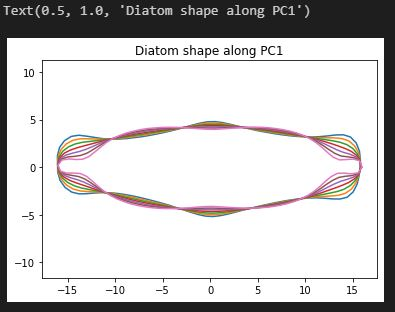
\includegraphics[width=0.75\textwidth]{Figures/Result_of_diatoms.JPG}
%     \caption{Plotted diatom}
% \end{figure}

